\documentclass[10pt]{beamer}

\usetheme[progressbar=frametitle]{metropolis}
\usepackage{appendixnumberbeamer}

\usepackage{booktabs}
\usepackage[scale=2]{ccicons}

\usepackage{pgfplots}
\usepgfplotslibrary{dateplot}

\usepackage{xspace}
\newcommand{\themename}{\textbf{\textsc{metropolis}}\xspace}

\usepackage{listings}

\colorlet{punct}{red!60!black}
\definecolor{background}{HTML}{EEEEEE}
\definecolor{delim}{RGB}{20,105,176}
\colorlet{numb}{magenta!60!black}
\definecolor{dkgreen}{rgb}{0,0.6,0}
\definecolor{ltgray}{rgb}{0.5,0.5,0.5}

\lstdefinelanguage{json}{
    basicstyle=\smallfont\ttfamily,
    numbers=left,
    numberstyle=\scriptsize,
    stepnumber=1,
    numbersep=1pt,
    showstringspaces=false,
    breaklines=true,
    frame=lines,
    backgroundcolor=\color{background},
    literate=
     *{0}{{{\color{numb}0}}}{1}
      {1}{{{\color{numb}1}}}{1}
      {2}{{{\color{numb}2}}}{1}
      {3}{{{\color{numb}3}}}{1}
      {4}{{{\color{numb}4}}}{1}
      {5}{{{\color{numb}5}}}{1}
      {6}{{{\color{numb}6}}}{1}
      {7}{{{\color{numb}7}}}{1}
      {8}{{{\color{numb}8}}}{1}
      {9}{{{\color{numb}9}}}{1}
      {:}{{{\color{punct}{:}}}}{1}
      {,}{{{\color{punct}{,}}}}{1}
      {\{}{{{\color{delim}{\{}}}}{1}
      {\}}{{{\color{delim}{\}}}}}{1}
      {[}{{{\color{delim}{[}}}}{1}
      {]}{{{\color{delim}{]}}}}{1},
}

\lstset{
  	backgroundcolor=\color{background},
  	basicstyle=\normalfont\ttfamily,
  	breakatwhitespace=false,
  	breaklines=true,
  	captionpos=b,
  	commentstyle=\color{dkgreen},
  	deletekeywords={...},
  	escapeinside={\%*}{*)},
  	extendedchars=true,
  	frame=single,
  	keepspaces=true,
  	keywordstyle=\color{blue},
  	language=SQL,
  	morekeywords={*,modify,MODIFY,...},
  	numbers=left,
  	numbersep=15pt,
  	numberstyle=\tiny,
  	rulecolor=\color{ltgray},
  	showspaces=false,
  	showstringspaces=false, 
  	showtabs=false,
  	stepnumber=1,
  	tabsize=4,
  	title=\lstname
}

\title{Master's thesis presentation}
\subtitle{Domain-Oriented Microservices Gateway Monitoring Using Big Data Techniques}
% \date{\today}
\date{24th, February 2022}
\author{Cristian M. Abrante Dorta}
\institute{Aalto University \& Unity Technologies}
%\titlegraphic{\hfill\includegraphics[height=1.5cm]{logo.pdf}}

\begin{document}

\maketitle

\begin{frame}{Table of contents}
  \setbeamertemplate{section in toc}[sections numbered]
  \tableofcontents%[hideallsubsections]
\end{frame}

\section{Introduction}

\begin{frame}{Microservices architecture}
    This architecture pattern has the following characteristics (Lewis et al. \cite{MicroservicesCharacteristics}):

    \begin{columns}
        \column{0.5\textwidth}
        \begin{figure}
            \centering
            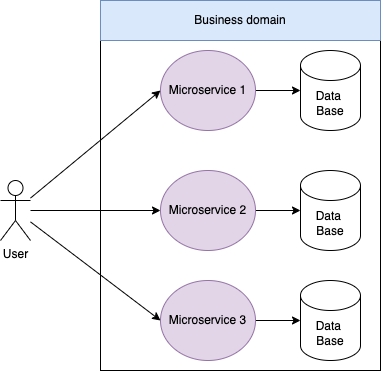
\includegraphics[width=0.7\textwidth]{src/thesis/img/literature-review/microservices.png}
            \caption{Diagram representing microservices architecture}
            \label{fig:my_label}
        \end{figure}
        
        \column{0.5\textwidth}
        \begin{itemize}
            \item \textbf{Modularity of services}
            \item \textbf{Orgnized around business capabilities}
            \item \textbf{They are product not projects}
            \item \textbf{Decentralized data governance}
        \end{itemize}
    \end{columns}
\end{frame}

\begin{frame}{Domain-Oriented Microservices Architecture}
    Introduced by Gluck A. \cite{DOMAUber}, it is composed by the following elements:\\
    \vspace{0.5cm}
    \begin{columns}
        \column{0.5\textwidth}
        \begin{figure}
            \centering
            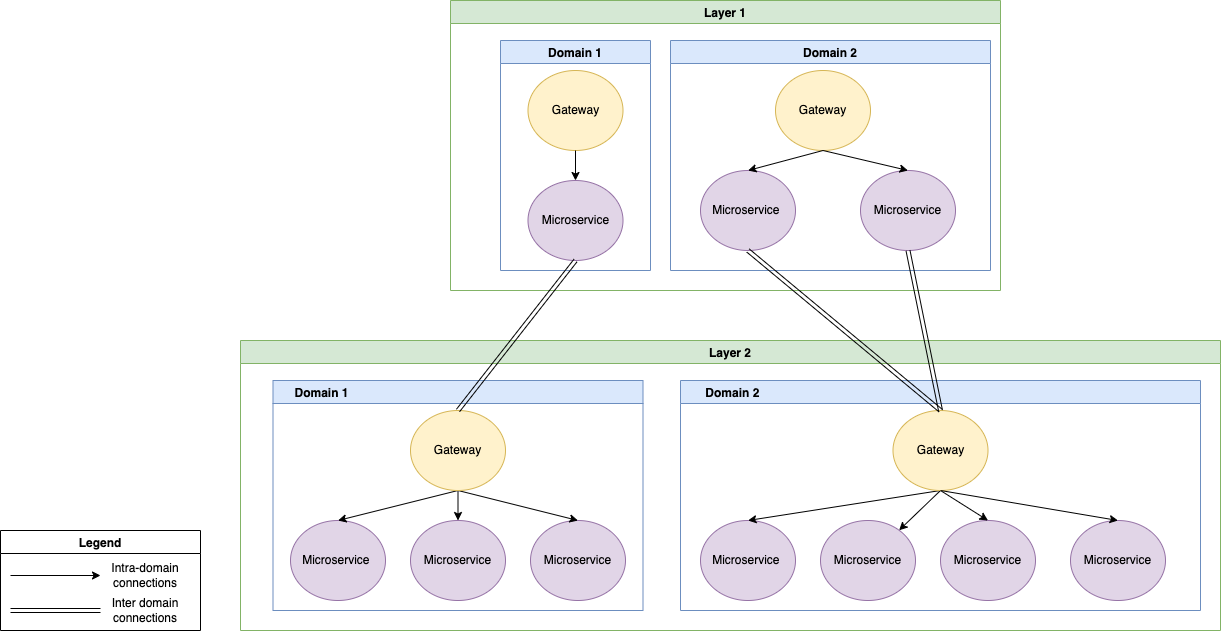
\includegraphics[width=\textwidth]{src/thesis/img/literature-review/doma.png}
            \caption{Diagram representing DOMA}
            \label{fig:my_label}
        \end{figure}
        
        \column{0.5\textwidth}
        \begin{itemize}
            \item \textbf{Domain}
            \item \textbf{Layers}
            \item \textbf{Gateway}
            \item \textbf{Extension architecture}
        \end{itemize}
    \end{columns}
    
    This architecture make sense in \textbf{big organizations} with hundreds of interconnected microservices.
\end{frame}

\begin{frame}{Company background}
    This project it is done in the context of the Acquire Unit of \textbf{UnityAds} product.
    
    \begin{figure}
        \centering
        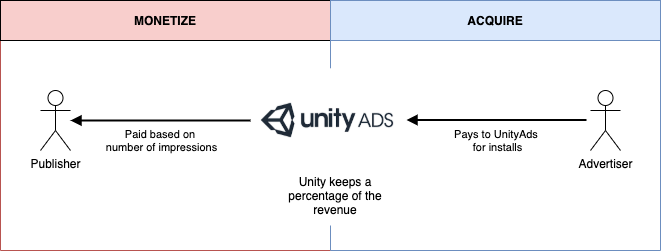
\includegraphics[scale=0.35]{src/thesis/img/background/unity-ads.png}
        \caption{Diagram representing the UnityAds advertisement network}
        \label{fig:unity-ads}
    \end{figure}
\end{frame}

\begin{frame}{Acquire Unit architecture}
    The Acquire Unit is a \textbf{DOMA} from the technical point of view.
    
    \begin{figure}
        \centering
        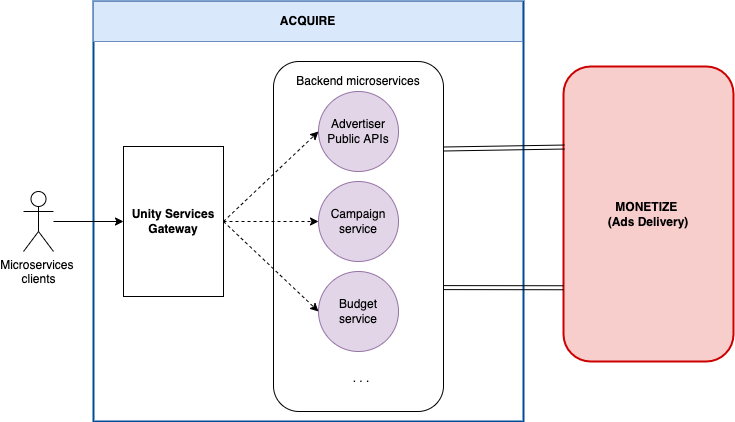
\includegraphics[scale=0.27]{src/thesis/img/background/acquire-division.png}
        \label{fig:my_label}
    \end{figure}
\end{frame}

\begin{frame}{DOMA Gateway}
    One of the main elements of DOMA is the gateway, which serves as the entry point for the domains. The gateway has to fulfil these high-level responsibilities (M. Thangavelu et al. \cite{UberGateway}):
    
    \begin{itemize}
        \item Auditing pipeline
        \item Identity
        \item Rate limiting
        \item Documentation
        \item Response field trimming
        \item Datacenter affinity
        \item Short-term user bans
    \end{itemize}
    
    On the company context, the gateway is the \textbf{Unity Services Gateway}.
\end{frame}

\section{Problem definition}

%%%%%%%%%%%%%%%%%%%%%%%%%%%%%%%%%%%%%%%%%%%%%%
% - Explain the different problems that the
%   stakeholders had.
% - Introduce the research questions.
%%%%%%%%%%%%%%%%%%%%%%%%%%%%%%%%%%%%%%%%%%%%%%

\begin{frame}{Problem definition}
    The gateway present some drawbacks on the visibility of the errors emitted by those high level responsibilities:
    \vspace{0.5cm}
    \metroset{block=fill}
    \begin{block}<1->{Advertiser public APIs Team}
        They should be aware of the errors that the advertisers are producing, and that are handled on the gateway side, e.g. rate limiting.
    \end{block}
    
    \begin{block}<2->{Product managers and client partners}
        They are responsible for the communication with the client so they should be aware on when the requests passing through the gateway are failing.
    \end{block}
    
    \begin{block}<3->{Security team}
        If any user is doing malicious usage of the APIs the security team has to be aware of it.
    \end{block}
\end{frame}

\begin{frame}{Research question}
    This lead to the three research questions addressed on this thesis:
    
    \begin{itemize}
    \item[\textbf{Q1}]<1-> \textit{What is the best way to represent the possible high-level errors that a DOMA gateway can produce?}
    \item[\textbf{Q2}]<2-> \textit{What is the optimal technology for storing the errors that a DOMA gateway can produce?}
    \item[\textbf{Q3}]<3-> \textit{How to correctly visualize and communicate with the stakeholders the errors a DOMA gateway can produce?}
\end{itemize}

\end{frame}

\section{Technical solution}

%%%%%%%%%%%%%%%%%%%%%%%%%%%%%%%%%%%%%%%%%%%%%%
% - Explain the defined gateway format.
% - Explain the error definition format. 
% - Explain the technical solution from the 
%   3 points of view:
% - Event gathering.
% - BigQuery setup
% - Pipeline creation from logs to storage.
% - Visualization dashboard
%%%%%%%%%%%%%%%%%%%%%%%%%%%%%%%%%%%%%%%%%%%%%%

\begin{frame}{Gateway configuration file}
    The way for doing the configuration is to compose a series of filters:
    
    \begin{itemize}
        \item \textbf{Auditing filter}
        \item \textbf{Identity filter}
        \item \textbf{Rate limit filter}
        \item \textbf{Documentation filter}
        \item \textbf{Response fields trimming}
    \end{itemize}
\end{frame}

\begin{frame}{Gateway configuration file}
    \begin{figure}
        \centering
        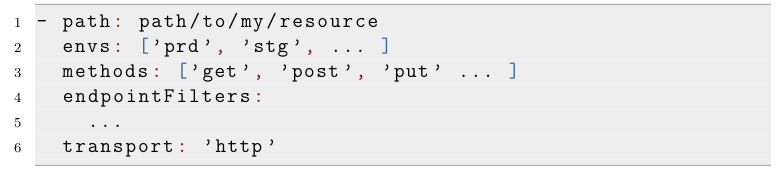
\includegraphics[scale=0.5]{src/presentation/img/config-general.png}
        \caption{General structure}
        \label{fig:my_label}
    \end{figure}
    
    \begin{columns}
        \column{0.5\textwidth}
        \begin{figure}
            \centering
            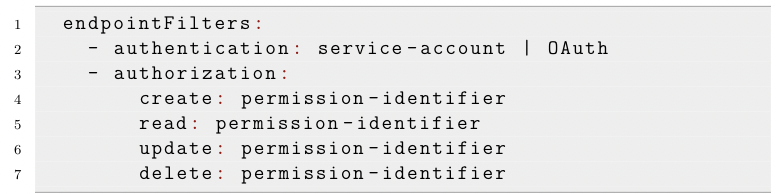
\includegraphics[width=\textwidth]{src/presentation/img/config-identity.png}
            \caption{Identity filter}
        \end{figure}
        
        \column{0.5\textwidth}
        \begin{figure}
            \centering
            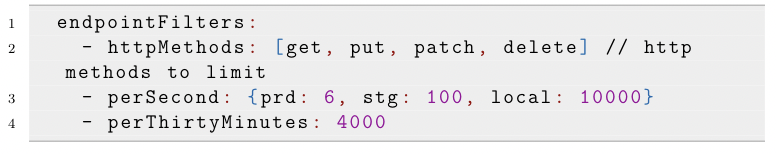
\includegraphics[width=\textwidth]{src/presentation/img/config-ratelimit.png}
            \caption{Rate-limit filter}
        \end{figure}
    \end{columns}
\end{frame}

\begin{frame}{Error events format}
    This format will define the errors that the gateway will emit in relation with its responsibilities.
    \vspace{0.5cm}
    \begin{columns}
        \column{0.5\textwidth}
        \onslide<1->
        \begin{table}[]
            \centering
            \begin{tabular}{|l|}
                \hline
                Common event fields     \\ \hline \hline
                \texttt{source}         \\ \hline
                \texttt{requestId}      \\ \hline
                \texttt{path}           \\ \hline
                \texttt{organizationId} \\ \hline
                \texttt{httpMethod}     \\ \hline
                \texttt{apiVersion}     \\ \hline
                \texttt{apiType}        \\ \hline
                \texttt{apiNamespace}   \\ \hline
                \texttt{timestamp}      \\ \hline
            \end{tabular}
        \end{table}
        
        \onslide<2->
        \column{0.5\textwidth}
        \begin{table}[]
            \centering
            \begin{tabular}{|l|}
                \hline
            Rate limit specific field   \\ \hline \hline
                \texttt{rateLimitReason}\\ \hline
                \texttt{quota}          \\ \hline
                \texttt{group}          \\ \hline
            \end{tabular}
        \end{table}
        \vspace{1.0cm}
        \centering
        \onslide<3->
        Other possible responsibility specific fields ...
    \end{columns}
\end{frame}

\begin{frame}{Data storage selection}
    
    The data storage selection has to be done according to \textbf{three criteria}:
    
    \begin{table}[h!]
        \centering
        \begin{tabular}{lccc}
            \toprule
           & C1 - Price    & C2 - Data Access & C3 - Integration \\ \midrule
BigQuery   & \$8.4/month   & Easy             & High \\
Amplitude  & Free          & Medium           & Medium  \\
PostgreSQL & \$109.9/month & Medium           & High  \\                \bottomrule
        \end{tabular}
\caption{Data storage technology}
        \label{tab:data-souces}
    \end{table}
    
    \centering
    Given those three criteria \textbf{BigQuery} is the selected technology.
\end{frame}

\begin{frame}{BigQuery setup}
    For doing the setup a new table is created using \textbf{Terraform} configuration, the result is the following on the UI:
    
    \begin{figure}
        \centering
        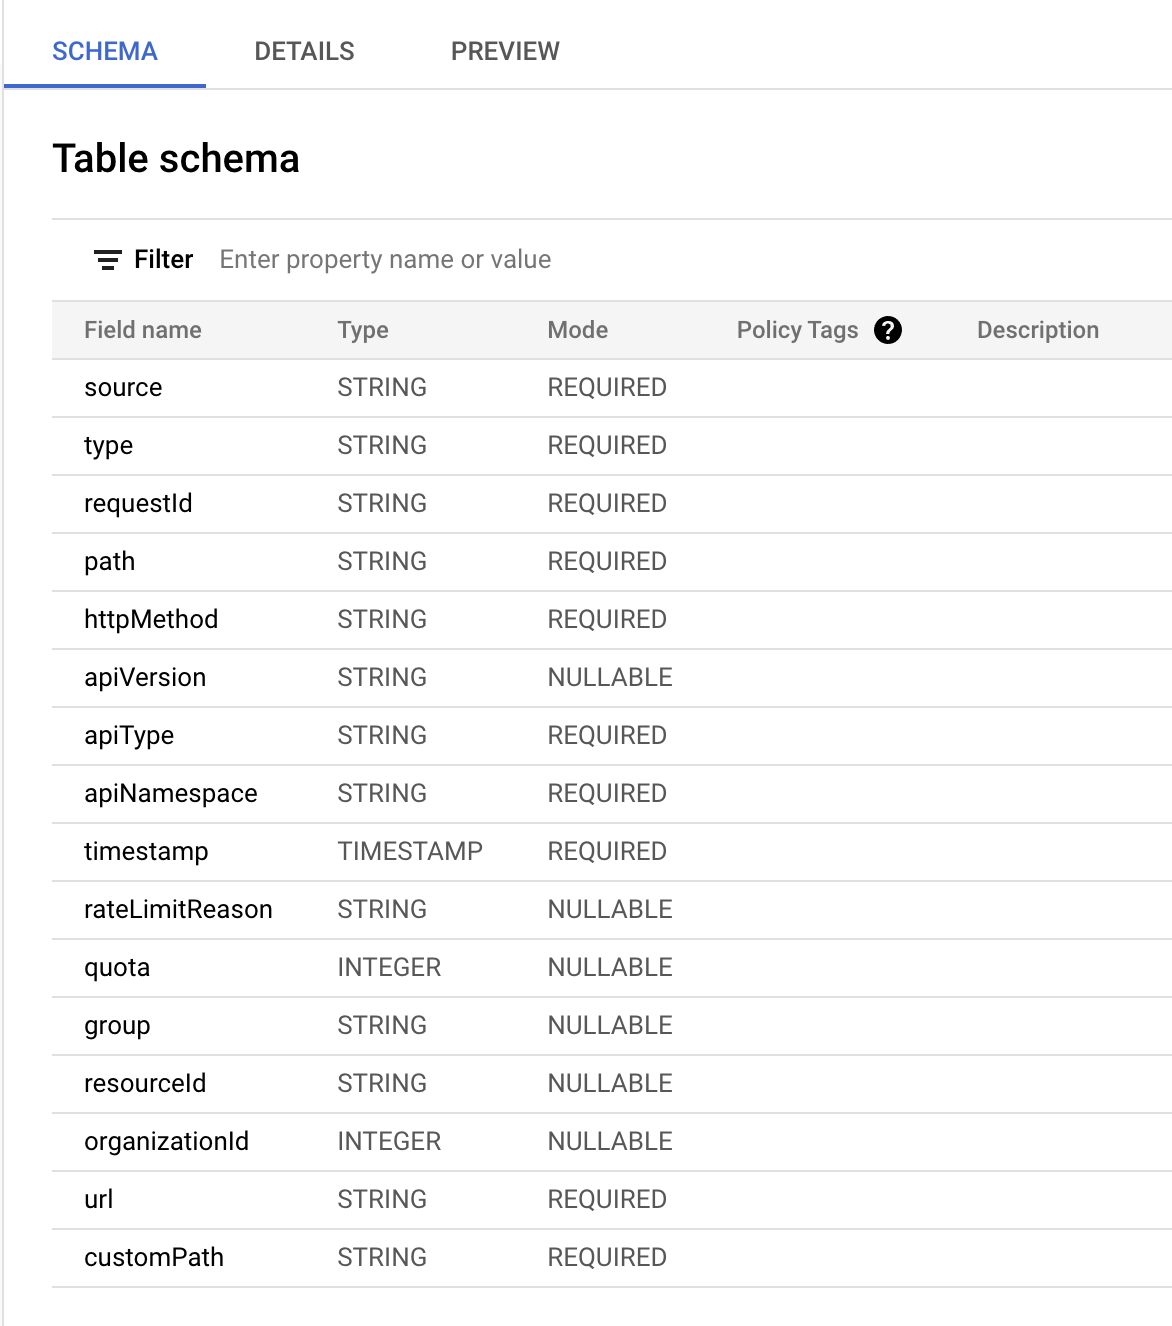
\includegraphics[scale=0.25]{src/thesis/img/technical-solution/bigquery-schema.png}
        \label{fig:my_label}
    \end{figure}
\end{frame}

\begin{frame}{Events gathering}
    The events gathering has to be placed on the events handlers of the \textbf{Unity Services Gateway}.
    
    \begin{figure}
        \centering
        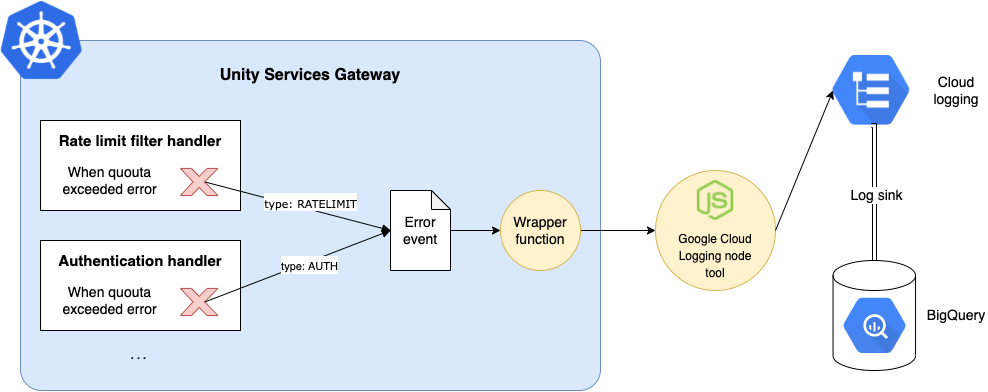
\includegraphics[scale=0.3]{src/thesis/img/technical-solution/events-gathering.png}
        \caption{Diagram showing the events workflow}
        \label{fig:my_label}
    \end{figure}
\end{frame}

\begin{frame}[fragile]{Log Sinks}
    Log sink allows the \textbf{persistance} on BigQuery of the logs emitted on the gateway side. It is done by appliying a Terraform configuration.
    \vspace{0.5cm}
    
    \begin{lstlisting}[language=json,firstnumber=1]
resource "google_project_sink" "log_sink" {
  name                   = var.sink_name
  destination  = "bigquery.googleapis.com/..."
  filter                 = var.filter
  unique_writer_identity = true

  bigquery_options {
    use_partitioned_tables = true
  }
}
    \end{lstlisting}
\end{frame}

\begin{frame}{Error visualization dashboard}
    The dashboard constructed using Grafana uses the \texttt{bigquery-grafana-plugin} to access the BigQuery datasource.
    \vspace{0.5cm}
    
    \begin{figure}
        \centering
        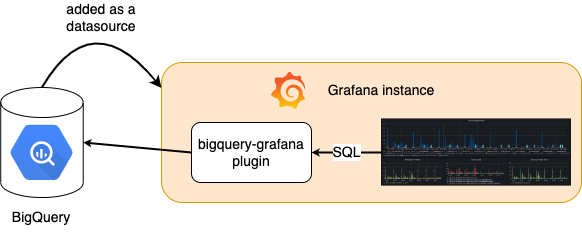
\includegraphics[scale=0.4]{src/thesis/img/technical-solution/grafana-connection.png}
    \end{figure}
\end{frame}

\begin{frame}{Error visualization dashboard}
    \centering
    \huge \textsc{Demo}
\end{frame}

\section{Evaluation}

%%%%%%%%%%%%%%%%%%%%%%%%%%%%%%%%%%%%%%%%%%%%%%
% - Comparison of the framework with the other
%   two open source gateways.
%%%%%%%%%%%%%%%%%%%%%%%%%%%%%%%%%%%%%%%%%%%%%%

\begin{frame}{Evaluation of the event gathering}
    For the evaluation of the event gathering \textbf{Jest} is used with mock servers and mock data.
    
    \begin{figure}
        \centering
        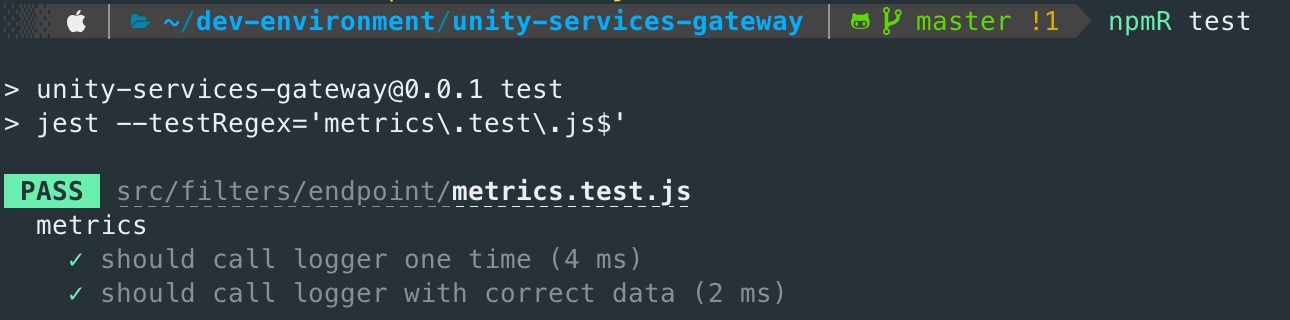
\includegraphics[scale=0.4]{src/presentation/img/jest.png}
    \end{figure}
\end{frame}


\begin{frame}{E2E evaluation}
    The method for the end-to-end evaluation consisted on doing \textbf{6.000} fake API calls to the services that are dependant on the gateway, on the staging environment.
    \vspace{0.5cm}
\begin{table}[]
    \centering
    \begin{tabular}{cccc}
    \toprule
         &  production & staging & local \\
    \midrule
    Rate Limit & 30 & 1000 & 3000 \\
    \bottomrule
    \end{tabular}
    \caption{Rate limit configuration}
    \label{tab:my_label}
\end{table}

    \metroset{block=fill}
    \begin{block}{Expected result (on staging)}
        5.000 rows should be stored on BigQuery, as the rate limit should be triggered for each call after the first 1.000.
    \end{block}
\end{frame}

\begin{frame}[fragile]{E2E evaluation}
    After that execution the query to the data source return the following value:
    
    \begin{figure}
        \centering
        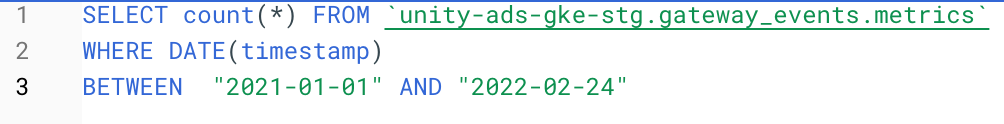
\includegraphics[scale=0.5]{src/presentation/img/bigquer-query.png}
        \caption{SQL query executed}
    \end{figure}
    
    \begin{columns}
        \column{0.5\textwidth}
        \begin{figure}
            \centering
            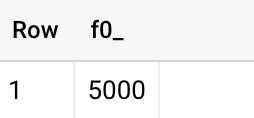
\includegraphics[width=0.6\textwidth]{src/presentation/img/bigquery-number.png}
            \caption{Number of rows retrieved}
            \label{fig:my_label}
        \end{figure}
        
        \column{0.5\textwidth}
        \begin{figure}
            \centering
            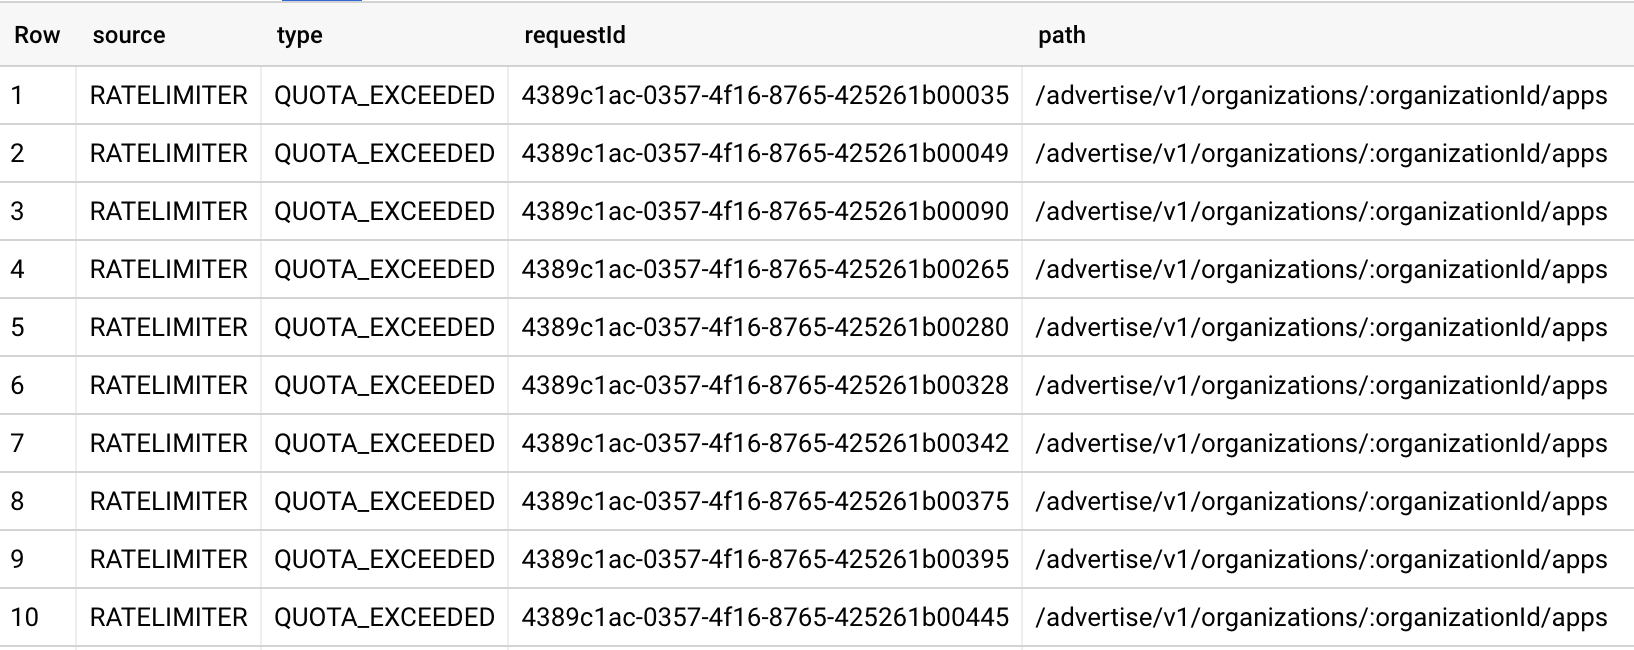
\includegraphics[width=\textwidth]{src/presentation/img/bigquery-rows.png}
            \caption{Subset of rows retrieved}
            \label{fig:my_label}
        \end{figure}
    \end{columns}
\end{frame}

\begin{frame}{Framework comparison}
    
    The solution is compared with other open source gateway According to three criteria
    
    \begin{itemize}
        \item[C1] High-level responsibilities matching to individual routes
        \item[C2] Error format definition
        \item[C3] Data storage selection
        \item[C4] Visualization of high-level errors
    \end{itemize}
    
    \onslide<2->
    \begin{table}[h]
\begin{tabular}{lllll}
\toprule
                  & \multicolumn{1}{c}{C1} & \multicolumn{1}{c}{C2} & \multicolumn{1}{c}{C3}        & \multicolumn{1}{c}{C4} \\
\midrule
Kong              & Yes - with UI           & No                      & Yes & No                      \\ \hline
Zuul              & Yes - with code         & Yes                     & No                             & No                      \\ \hline
\textbf{Proposed solution} & Yes - with file         & Yes                     & Yes - BigQuery                 & Yes                     \\
\bottomrule
\end{tabular}
\caption{Framework comparison table}
\label{tab:frameworks}
\end{table}
    
\end{frame}

\section{Conclusion and future work}

%%%%%%%%%%%%%%%%%%%%%%%%%%%%%%%%%%%%%%%%%%%%%%
% - Offer a conclussion from the three 
%   different points of view depending on the
%   organization size.
% - Explain the future work same as in the 
%   thesis document.
%%%%%%%%%%%%%%%%%%%%%%%%%%%%%%%%%%%%%%%%%%%%%%

\begin{frame}{Conclussions}
    \metroset{block=fill}
    \begin{block}{}
        The solution has been satisfactory for all the stakeholders and has been used for identifying some problems with their integration.
    \end{block}
    
    \onslide<2->
    Depending on the size of the organization the possibilities for implementing this solution for gateway monitoring.
    
    \begin{itemize}
        \item<3-> \textbf{Startups}: on those organizations there is usually no need to have a DOMA, so the monitoring is not needed.
        \item<4-> \textbf{Mid-size organizations}: On those, the gateway monitoring might be needed, but maybe with simpler options like Amplitude.
        \item<5-> \textbf{Multinational companies}: On those this type of solutions might be suitable due to the high number of teams and microservices.
    \end{itemize}
\end{frame}

\begin{frame}{Future work}
    There are three improvement ideas that can be applied to this project:
    
    \begin{itemize}
        \item<1-> Extend error object to support more types of errors.
        \item<2-> Create a composable gateway logic.
        \item<3-> Create a plugin that will pack the solution for being used in one of the standard gateways.
    \end{itemize}
\end{frame}

\begin{frame}[allowframebreaks]{References}

  \bibliography{presentation}
  \bibliographystyle{abbrv}

\end{frame}

\begin{frame}[standout]
    Thank you very much for your attention!\\
    Any questions?
\end{frame}

\end{document}
